\begin{table}[H]
\centering
\caption{Descomposición de la variación en la remuneración laboral, 2010--2025}
\label{tab:descomposicion_remuneracion_educacion}
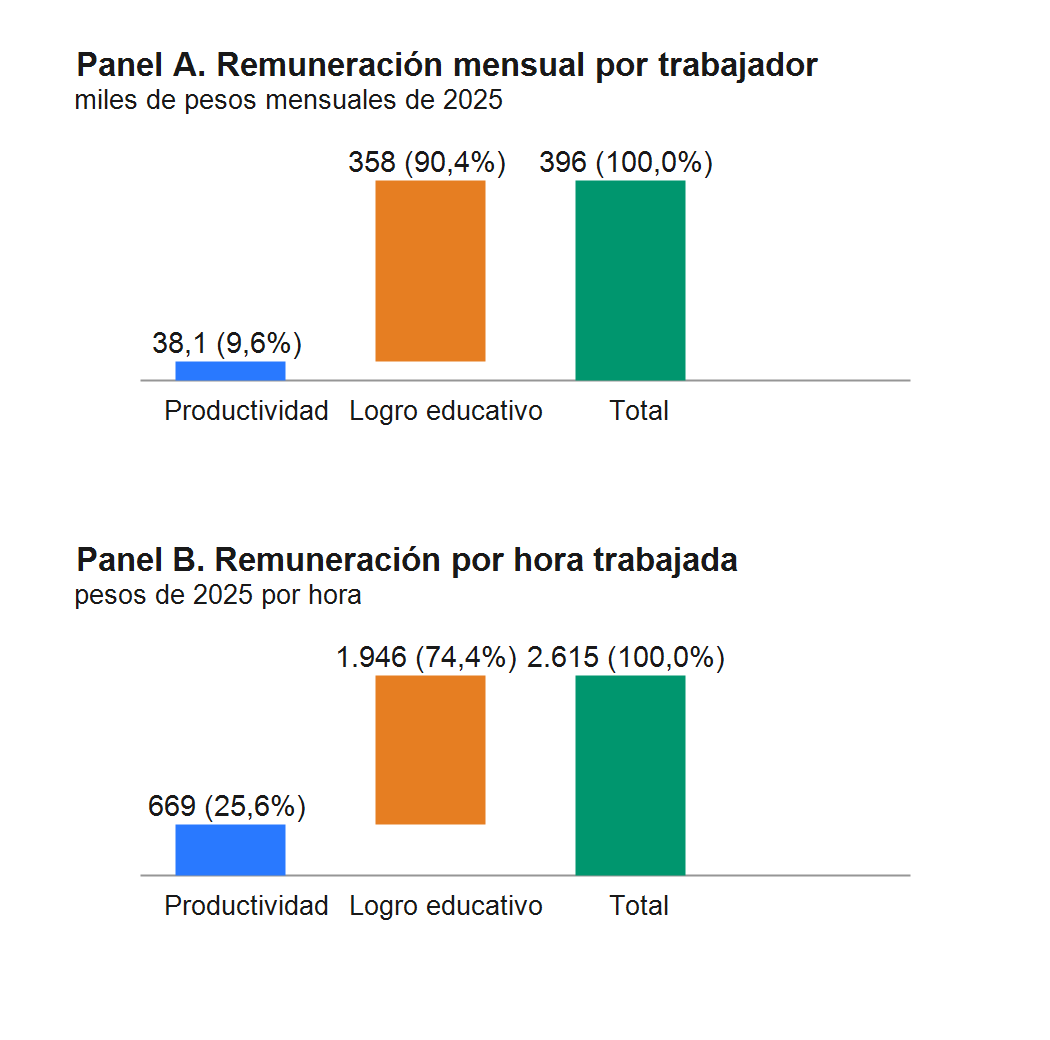
\includegraphics[width=0.98\textwidth]{Paper/figures/fig_descomposicion_remuneracion_educacion_cascada.png}
\caption*{\footnotesize %Nota: el Panel A mide la variación de la remuneración mensual por trabajador en miles de pesos de 2025. El Panel B mide la variación de la remuneración por hora trabajada en pesos de 2025 por hora. ``Mayor productividad de cada logro educativo'' mide el aporte de los cambios de remuneración dentro de cada logro educativo. ``Mayor logro educativo de la población ocupada'' mide el aporte de los cambios en el peso relativo de esos logros. La descomposición usa los ponderadores promedio de 2010 y 2025. 
Fuente: cálculos propios con GEIH del DANE.}
\end{table}
